\documentclass[12pt,a4paper]{scrartcl}
\usepackage[utf8]{inputenc}
\usepackage[english]{babel}
\usepackage{amsmath}
\usepackage{amsfonts}
\usepackage{amssymb}
\usepackage{enumerate}
\usepackage{listings}
\usepackage{pdfpages}
\usepackage{textcomp}
\usepackage{url}
\usepackage{comment}
\usepackage{xspace}
\usepackage{dirtree}
\usepackage{enumitem}
\usepackage{todonotes}
\usepackage{framed}
\usepackage{pifont}% http://ctan.org/pkg/pifont
\newcommand{\cmark}{\ding{51}}%
\newcommand{\xmark}{\ding{55}}%

% ONLY FOR DRAFT MODE
% \usepackage[right=6cm,marginparwidth=5cm]{geometry}

\newcommand{\intrudy}{\textsc{Intrudy}\xspace}
\newcommand{\rospy}{\texttt{rospy}\xspace}
\newcommand{\marginnote}[1]{\marginpar{\scriptsize\color{blue}{#1}}}
\newcommand{\degrees}{\textdegree\xspace}
\newenvironment{algorithmframe}
{\begin{tabular}{|p{0.95\textwidth}}}%
{\end{tabular}}


%%%%%% EPYDOC-GEN
\usepackage{alltt, parskip, fancyhdr, boxedminipage}
\newcommand{\pysrcexcept}[1]{\textcolor{py@exceptcolour}{\small\textbf{#1}}}
\newlength{\funcindent}
\newlength{\funcwidth}
\setlength{\funcindent}{1cm}
\setlength{\funcwidth}{\textwidth}
\addtolength{\funcwidth}{-2\funcindent}
\newlength{\varindent}
\newlength{\varnamewidth}
\newlength{\vardescrwidth}
\newlength{\varwidth}
\setlength{\varindent}{1cm}
\setlength{\varnamewidth}{.3\textwidth}
\setlength{\varwidth}{\textwidth}
\addtolength{\varwidth}{-4\tabcolsep}
\addtolength{\varwidth}{-3\arrayrulewidth}
\addtolength{\varwidth}{-2\varindent}
\setlength{\vardescrwidth}{\varwidth}
\addtolength{\vardescrwidth}{-\varnamewidth}
%%%%%%


\usepackage{hyperref}
\hypersetup{
    colorlinks,
    citecolor=black,
    filecolor=black,
    linkcolor=black,
    urlcolor=black
}

\usepackage{float}
\floatstyle{boxed}
\restylefloat{figure}

\begin{document}

\begin{titlepage}
\begin{center}

\newcommand{\HRule}{\rule{\linewidth}{0.5mm}}

% Upper part of the page. The '~' is needed because \\
% only works if a paragraph has started.
%\includegraphics[width=0.15\textwidth]{./logo}~\\[1cm]

\textsc{\LARGE University of Bonn}\\[0.5cm]

\includegraphics[width=0.35\textwidth]{img/unilogo.pdf}
\\[1.5cm]
\textsc{Lab Course Mobile Robots (MA-INF 4310)}
\\[1.5cm]
% Title
\HRule \\[0.8cm]
\textsc{\Large INTRUDY: The Intruder Detection and Following System}\\[0.5cm]
{ \huge \bfseries Programmer's Manual \\[0.4cm] }

\HRule \\[1.5cm]

% Author and supervisor

\begin{minipage}{0.4\textwidth}
\begin{flushleft} \large
\textbf{Authors:}\\
Pablo \textsc{Aponte} \\
Ilya \textsc{Manyugin} 
\end{flushleft}
\end{minipage}
\begin{minipage}{0.4\textwidth}
\begin{flushright} \large
\textbf{Supervisor:} \\
Dr.~Nils \textsc{Goerke}
\end{flushright}
\end{minipage}

\null
\vfill

\textsc{Bonn, 2013}
\end{center}
\end{titlepage}

\tableofcontents
\newpage

% PREFACE
\phantomsection
\addcontentsline{toc}{section}{Preface}
\section*{Preface}
	\label{sec:preface}
	This document describes \intrudy, The Intruder Detection and Following System. The emphasis of this document is made on the software part of \intrudy, with some introduction of the underlying theoretical concepts and the description of the hardware platform.
% section preface (end)


% GENERAL DESCRIPTION
\section{General Description} % (fold)
	\label{sec:general_description}


	\subsection{Hardware Platform} % (fold)
	\label{sub:hardware_platform}

		\intrudy is run upon the \textsc{RoomRider}, the teaching and research mobile robot platform developed by the Department of Autonomous Intelligent Systems (Informatik VI) at the University of Bonn \cite[III.A. Roomrider]{goerke2009}.\\
		The platform itself is based on the iRobot 530 Roomba Vacuuming Robot. Additionally it features a SICK S300 laser scanner and a notebook, enabling the control of the robot's movements via the serial interface.\\ 
		The laser scanner supports a scanning azimuth of 270\degrees covering the range from -135\degrees to +135\degrees, where 0\degrees is the frontal point of the platform. The laser scanner data is available with a resolution of 0.5\degrees as an array of 540 values. The range measured by the scanner to the obstacle can vary from 5 cm to 30 m.

	% subsection hardware_platform (end)

	\subsection{Software Platform} % (fold)
	\label{sub:software_platform}

		In the software part the Robot Operating System (ROS) was used as the main software framework for the software development controlling the robot\cite{ROSmain}. ROS provides many services to ease the development and testing of the software written for different kinds of robots, among these services are hardware abstraction and transport of the messages between processes ("nodes" in ROS terminology). The Robot Operating System is a flexible framework for writing robot software \cite{ROSmain}. It provides a set of tools and libraries for programming complex robot behavior, and allows for an operating system. ROS is distributed under a BSD free software licence.

		For the purpose of this work, the Long-Term Support release of Ubuntu Linux 10.04.2 Lycid Lynx was used as the main operating system running on the notebook, and the ROS Elecrtic distribution was ran in that environment.

		ROS supports packaging as a mean of distribution of its components, and the two main ROS packages used in our work are \texttt{roomrider\_driver} and \texttt{sicks300}. 
		The roomrider driver package is a driver used to control the RoomRider platform and to get the sensory information via the serial interface of the Roomba \cite{ROSRoomrider}. The sicks300 package is a driver that reads the scan data of a Sick S300 Professional Laser Scanner via its serial interface \cite{ROSSicks}.
		Both packages were developed within the Autonomous Intelligent Systems Department at the University of Bonn.

		ROS provides a choice of three programming language bindings (so-called `client libraries' in ROS terminology): \texttt{roscpp} for C++ development, \texttt{rosjava} for Java and \rospy for Python bindings. In this work we chose to use Python programming language and the \rospy client API for the development of \intrudy, because of the flexibility and the ease of prototyping this language provides. Also, Python has a renown and extensive scientific library \texttt{scipy}, which provides a large set of high-level mathematical functions and allows for faster computations, as parts of it are written in plain C. This allows us to reduce the gap between the choice of the Python and the C++ client libraries.

	% subsection software_platform (end)

% section general_description (end)

\newpage

\section{The \intrudy ROS Package} % (fold)
\label{sec:intrudy_ros_package}

	\subsection{Running \intrudy} % (fold)
	\label{sub:running_intrudy}
	Since the code was written in Python there is no need to compile anything. To run it, the roslaunch command is used:


	\texttt{roslaunch intrudy intrudy.launch}


	It is important to note that \texttt{intrudy.py} in the \texttt{scripts} folder must have file system permissions to be read and executed.
	
	The node description of the \intrudy is as following:

	\texttt{<node pkg="intrudy" type="intrudy.py" output="screen" name="intrudy" ></node>}
	% subsection running_intrudy (end)

	\subsection{Package Structure} % (fold)
	\label{sub:package_structure}

		As briefly described in section~\ref{sub:software_platform}, \intrudy is written in Python programming language using the ROS Python client library; this architectural desicion also affects the way the ROS package is organized.
		
		\intrudy is distributed as a ROS package, a directory tree of a special structure. As the official documentation  \cite{ROSPackages} states, a ROS package can \textit{contain ROS nodes, a ROS-independent library, a dataset, configuration files, a third-party piece of software, or anything else that logically constitutes a useful module.}

		The \intrudy package directory tree is shown in Figure~\ref{fig:package_directory_structure}.

		\begin{figure}[htc]
			\dirtree{%
			.1 intrudy.
			.2 CMakeLists.txt\DTcomment{CMake build file}.
			.2 mainpage.dox\DTcomment{Doxygen mainpage documentation}.
			.2 Makefile.
			.2 manifest.xml\DTcomment{Package Manifest}.
			.2 launch\DTcomment{Roslaunch launch scenarios directory}.
			.3 intrudy.launch\DTcomment{Main launch file}.
			.3 intrudy\_sim.launch\DTcomment{Simulation launch file}.
			.2 scripts\DTcomment{Executable scripts (Python code) directory}.
			.3 controller.py\DTcomment{Intrudy controller}.
			.3 config.py\DTcomment{Intrudy configuration file}.
			.3 icp.py\DTcomment{The ICP module}.
			.3 intrudy.py\DTcomment{Intrudy main module}.
			.3 record.py\DTcomment{The Logging module}.
			.3 tracking.py\DTcomment{The Tracking module}.
			}
			\caption{\intrudy package directory tree}
			\label{fig:package_directory_structure}
		\end{figure}

	% subsection package_structure (end)

\subsection{Robot Steering Module} % (fold)
\label{sub:FSM}
	The movements of the robot are driven by the data that is returned by the target tracking module described in the section~\ref{sub:the_tracking_module}. In order to aid more smooth movements of the robot and to impelemnt the target re-acquisition, a Finite State Machine (FSM) was implemented within the program. 

	This FSM has four internal states, as following:
	\begin{enumerate}%[itemsep=0pt,topsep=0pt]
		\item \textit{Surveillance} \\
		In this state \intrudy is stationary (i.e., the command given on each iteration is $\{0, 0\}$, that is, both the linear and angular speeds are set to zero), and the movement detection threshold in the target tracking module is set to a lower value, in order to aid early target detection.

		\item \textit{Following} \\
		In this state \intrudy is moving, following a target, and the effective command is dependent on both the angle of the target relative to \intrudy's front and the distance between the \intrudy and the target.
		
		\item \textit{Re-Acquisition}\\
		The FSM transits to this state from the Following state if the Tracking Module reports a target loss (i.e., the return value of the \texttt{track} method is \texttt{None}).\\
		In this state \intrudy is still moving towards the place where the target was last detected, simultaneously trying to re-acquire the target. If \intrudy fails to re-acquire target within 5 time steps (a configurable parameter of \intrudy specified in \texttt{config.py}) since the target loss, it transits to the Surveillance state. If the target was successfully re-acquired, it transits to the Following state. 
		
		\item \textit{Collision}\\
		A collision detection algorithm ensures that all the range values retrieved from the SICK S300 laser scanner are greater than 0.15 m. If this assertion doesn't hold, we say that we detected a collision with an obstacle, and \intrudy transits into the Collision state. In this state \intrudy runs at each time step the collision detection algorithm in order to check, whether the obstacle has changed its location. Therefore, if \intrudy collides with a stable object, it cannot resolve the collision by itself, and the only way to make it operable again is for the user to move the robot away from the obstacle.
	\end{enumerate}

	These four states, as well as the transition paths between them, are shown in Figure~\ref{fig:intrudy_fsm_states}. In the figure, $t$ is the target, either \textit{None}, or $(\phi, r)$ meaning the angle and the distance to the target in polar coordinate system, respectively.

	\begin{figure}[htc]
	\center
	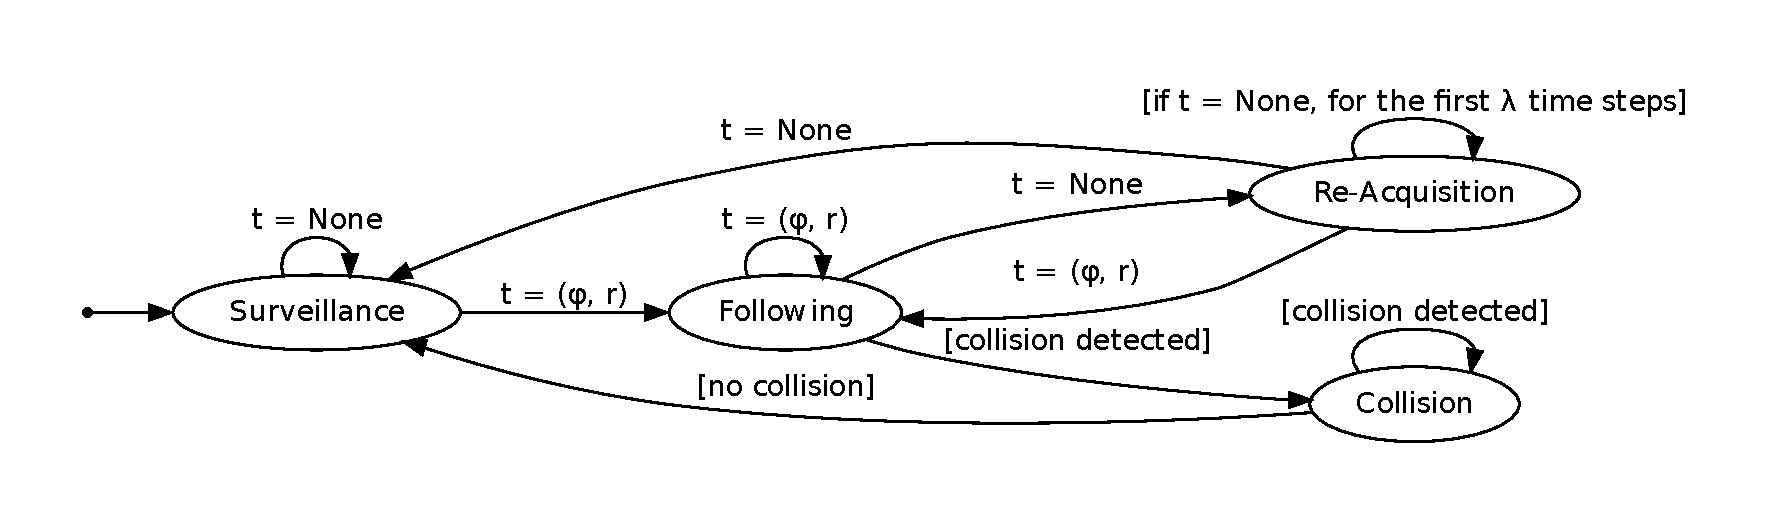
\includegraphics[width=\textwidth]{img/fsm.pdf}
	\caption{\intrudy internal FSM states}
	\label{fig:intrudy_fsm_states}
	\end{figure}

\subsection{Movement Detection and The Iterative Closest Point Algorithm} % (fold)
\label{sub:the_iterative_closest_point_algorithm}

The Iterative Closest Point (ICP) algorithm is a point set registration algorithm\cite{ICP1992}. In this work we employ ICP as a powerful algorithm for calculating the displacement of the objects between two raw scans made by the SICK S300 laser scanner.

The input of the ICP algorithm consists of the two sets of points (point clouds) from the raw scans, $X$ and $P$, where $X$ is the first scan, also called the \textit{source}, and $P$ is the second scan called the \textit{target}. The key idea of this algorithm is to find a correspondence between these two sets by finding the transformation (rotation $R$ and translation $t$) needed to transform the first set into the other, such that the sum of the squared error $E$, as shown in Formula~\ref{eq:icp_squared_error}, is minimized.
\begin{equation} \label{eq:icp_squared_error}
E(R, t) = \frac{1}{\left|P\right|} \sum^{\left|P\right|}_{i=1} (x_i - R \cdot p_i -  t)^2
\end{equation}
That is, this iterative algorithm keeps the \textit{target} cloud fixed, while it transforms the \textit{source} cloud, calculating the squared error (\ref{eq:icp_squared_error}) and comparing it to an arbitrary threshold, e.g. 0, until converged.

The main steps of the algorithm are as following:\\
\begin{algorithmframe}
\begin{enumerate}[itemsep=0pt,topsep=0pt]
	\item Find the correspondence between points: for each point in $X$ find the closest point in $P$.
	\item Find the correlation matrix between the new set and the corresponding points.
	\item Do an Singular Value Decomposition (SVD) to obtain the matrices necessary for the formula of the rotation matrix.
	\item Obtain the translation vector using the rotation matrix and the mean of the two sets.
	\item Apply both the rotation and translation matrix.
	\item Recalculate the mean squared error (Formula~\ref{eq:icp_squared_error}) and check if it is below the threshold, else go to step 1.
\end{enumerate}
\end{algorithmframe}

In the \intrudy project we implement and widely use a technique called the ICP Optimization. The main idea of the ICP Optimization is to use the ICP algorithm and previous knowledge about the target (its position), in order to reduce the search space in the newly obtained scan.

Given two scans $s_0$ and $s_1$, we apply the ICP algorithm using both of them, changing $s_0$ in such a way that the static objects (such as walls, chairs, etc.) remain in the same position in both scans, while the displaced objects (e.g., a person walking) are the ones that change between scans. We get the transformation $T$ as the output of the ICP algorithm, and we apply this transformation to the $s_0$ scan and the previously obtained target position $p_t$. Applying the transformation $T$ to the previous target position $t_p$, we get the estimation of the target in the next scan $p_{t}^{\prime} = T(p_t)$. This estimation is saved for later use in a class variable.

% subsection the_iterative_closest_point_algorithm (end)

\subsection{The Tracking Module} % (fold)
\label{sub:the_tracking_module}
The Tracking Module is arguably the most important part of \intrudy. This module allows the robot to track the target's position and follow it. The overall principle of functioning of the Tracking Module can be descbribed as follows.

\begin{enumerate}
	\item Given two range scans, we truncate the values to the maximum range $R_{max}$ (configurable parameter of the system), that is, for each distance $d_i$ in each of the scans, if $d_i > R_{max}$, then $d_i \gets R_{max} $. Additionaly the scans are converted from a robot-centric polar coordinate system into Cartesian coordinate system.
	If \intrudy is not in \textit{surveillance mode} (see section~\ref{sub:FSM} for the list of \intrudy modes), the ICP optimization of the first scan is done and, at the same time, the previously detected target, if any, is moved accordingly to this ICP optimization (see section~\ref{ssub:icp_optimization}). This optimization is done in the first scan so that we can also recalculate the position of the previously obtained target.

	\item After the optimization, the corresponding points are found in the two sets (scans). These are the points that are considered to have been a subject to transformation due to the target movement. 
	We consider all the $n$ points of the `new' scan $S_1$ and compute the Euclidean distance $E_d$ between each point from $S_1$ and all the points from the set $S_0$. If all the Euclidean distances are greater than a configurable parameter alpha, then the point $p_{S_1, i}$ is considered an `outlier' (see Formula~\ref{eq:icp_outlier}).
	
	\begin{equation} 
	\label{eq:icp_outlier}
	\forall p_{S_1, i} \in S_1, \forall p_{S_0, j} \in S_0, E_d(p_{S_0, j}, p_{S_1, i}) > \alpha
	\end{equation}

	This approach allows us to ignore the noise encountered in the data that is introduced by the resolution of the laser scanner, if the variance introduced by the noise is less than $\alpha$.

	\item After the outliers are found, it is necessary to find the difference between scans $S_0$ and $S_1$ in those points; thus we obtain the set of differences $D$. If each difference $d_i \in D$ is too small, it is considered to be noise and will be discarded. Then, the outliers are grouped together if they are situated in the neighboring range values in the scan (e.g., $\{p_{S_1, 50}, p_{S_1, 51}, \dots, p_{S_1, 70}\})$, and if they are of the same sign in the difference (either $d_i \geq 0$ or $d_i<0$). 

	Once the groups are formed, the most probable target position will be found. For this, the differences of the outliers should be considered. The predicted movement can be of three different types:
	\begin{itemize}
	\item all positive differences, meaning the target moved towards the robot, i.e., $\Delta y < 0, \Delta x = 0$;
	\item all negative differences, meaning the target moved away from the robot, i.e., $\Delta y > 0, \Delta x = 0$;
	\item combination of positive and negative differences, meaning $\Delta x \neq 0$.
	\end{itemize}
	The groups are thresholded by their size, the ones whose size is less than $\beta$ are filtered out.

	\item Once the most probable targets are found, we use a heuristic to determine which target is the best, and, therefore, the actual target the algorithm returns. 
	The heuristic selects that target, which is the closest one to the previous target location, determined in the previous run. If there is no previous target location, the algorithm will select the target consistion of the greatest number of points.

	If the robot is in either the \textit{following} or the \textit{re-aquisition} state, it will not use the full range of its lasers, but instead only a 90\degrees window centered in the previous target location. 

	While in this states, the target position will be also updated (transformed) to account for the robots movements.
\end{enumerate}

% subsection the_tracking_module (end)

% section intrudy_ros_package (end)

\newpage

\section{Source Code Documentation} % (fold)
\label{sec:source_code_documentation}

Each class of the \intrudy system is well documented, the style of the comments is compliant with the Epytext markup language and the full API reference, as well as the introspect of the modules can be generated with the Epydoc documentation generator. It supports many output formats, among them HTML, PDF and \LaTeX.

An example Epydoc output for the \intrudy code is shown below.

\begin{algorithmframe}
\subsection*{Functions}

    \label{controller:debug_info}
    \index{controller \textit{(module)}!controller.debug\_info \textit{(function)}}

    \vspace{0.5ex}

\hspace{.8\funcindent}\begin{boxedminipage}{\funcwidth}

    \raggedright \textbf{debug\_info}(\textit{msg})

    \vspace{-1.5ex}

    \rule{\textwidth}{0.5\fboxrule}
\setlength{\parskip}{2ex}
    Debug message function

\setlength{\parskip}{1ex}
    \end{boxedminipage}

    \label{controller:enum}
    \index{controller \textit{(module)}!controller.enum \textit{(function)}}

    \vspace{0.5ex}

\hspace{.8\funcindent}\begin{boxedminipage}{\funcwidth}

    \raggedright \textbf{enum}(**\textit{enums})

    \vspace{-1.5ex}

    \rule{\textwidth}{0.5\fboxrule}
\setlength{\parskip}{2ex}
    A function creating new type alike to the enum in C

\setlength{\parskip}{1ex}
    \end{boxedminipage}



\subsection*{Methods}

    \vspace{0.5ex}

\hspace{.8\funcindent}\begin{boxedminipage}{\funcwidth}

    \raggedright \textbf{\_\_init\_\_}(\textit{self})

    \vspace{-1.5ex}

    \rule{\textwidth}{0.5\fboxrule}
\setlength{\parskip}{2ex}
    Constructor

\setlength{\parskip}{1ex}
      Overrides: object.\_\_init\_\_

    \end{boxedminipage}

    \label{intrudy:IntRudy:laser_callback}
    \index{intrudy \textit{(module)}!intrudy.IntRudy \textit{(class)}!intrudy.IntRudy.laser\_callback \textit{(method)}}

    \vspace{0.5ex}

\hspace{.8\funcindent}\begin{boxedminipage}{\funcwidth}

    \raggedright \textbf{laser\_callback}(\textit{self}, \textit{data})

    \vspace{-1.5ex}

    \rule{\textwidth}{0.5\fboxrule}
\setlength{\parskip}{2ex}
    Laser callback called by the subscriber

\setlength{\parskip}{1ex}
    \end{boxedminipage}

    \label{intrudy:IntRudy:main_loop}
    \index{intrudy \textit{(module)}!intrudy.IntRudy \textit{(class)}!intrudy.IntRudy.main\_loop \textit{(method)}}

    \vspace{0.5ex}

\hspace{.8\funcindent}\begin{boxedminipage}{\funcwidth}

    \raggedright \textbf{main\_loop}(\textit{self})

    \vspace{-1.5ex}

    \rule{\textwidth}{0.5\fboxrule}
\setlength{\parskip}{2ex}
    Main execution loop

\setlength{\parskip}{1ex}
    \end{boxedminipage}

\\

\normalsize{\textbf{\textit{Inherited from object}}}

\begin{quote}
\_\_delattr\_\_(), \_\_format\_\_(), \_\_getattribute\_\_(), \_\_hash\_\_(), \_\_new\_\_(), \_\_reduce\_\_(), \_\_reduce\_ex\_\_(), \_\_repr\_\_(), \_\_setattr\_\_(), \_\_sizeof\_\_(), \_\_str\_\_(), \_\_subclasshook\_\_()
\end{quote}

\end{algorithmframe}


% section source_code_documentation (end)

\newpage

\section{Evaluation of Results} % (fold)
\label{sec:evaluation_of_results}

	\subsection{Tests Setup and Description} % (fold)
	\label{sub:tests_setup_and_description}

	After several qualitative tests in the simulator and on the real robot, it was concluded that the system should be tested in nine different setups. 

	The first four tests where done in a controlled enviroment, where several plywood boards worked as the walls. Figure~\ref{fig:test_setup} shows the first test setup and the enviroment described before.
	
	\begin{figure}[htc]
		\center
		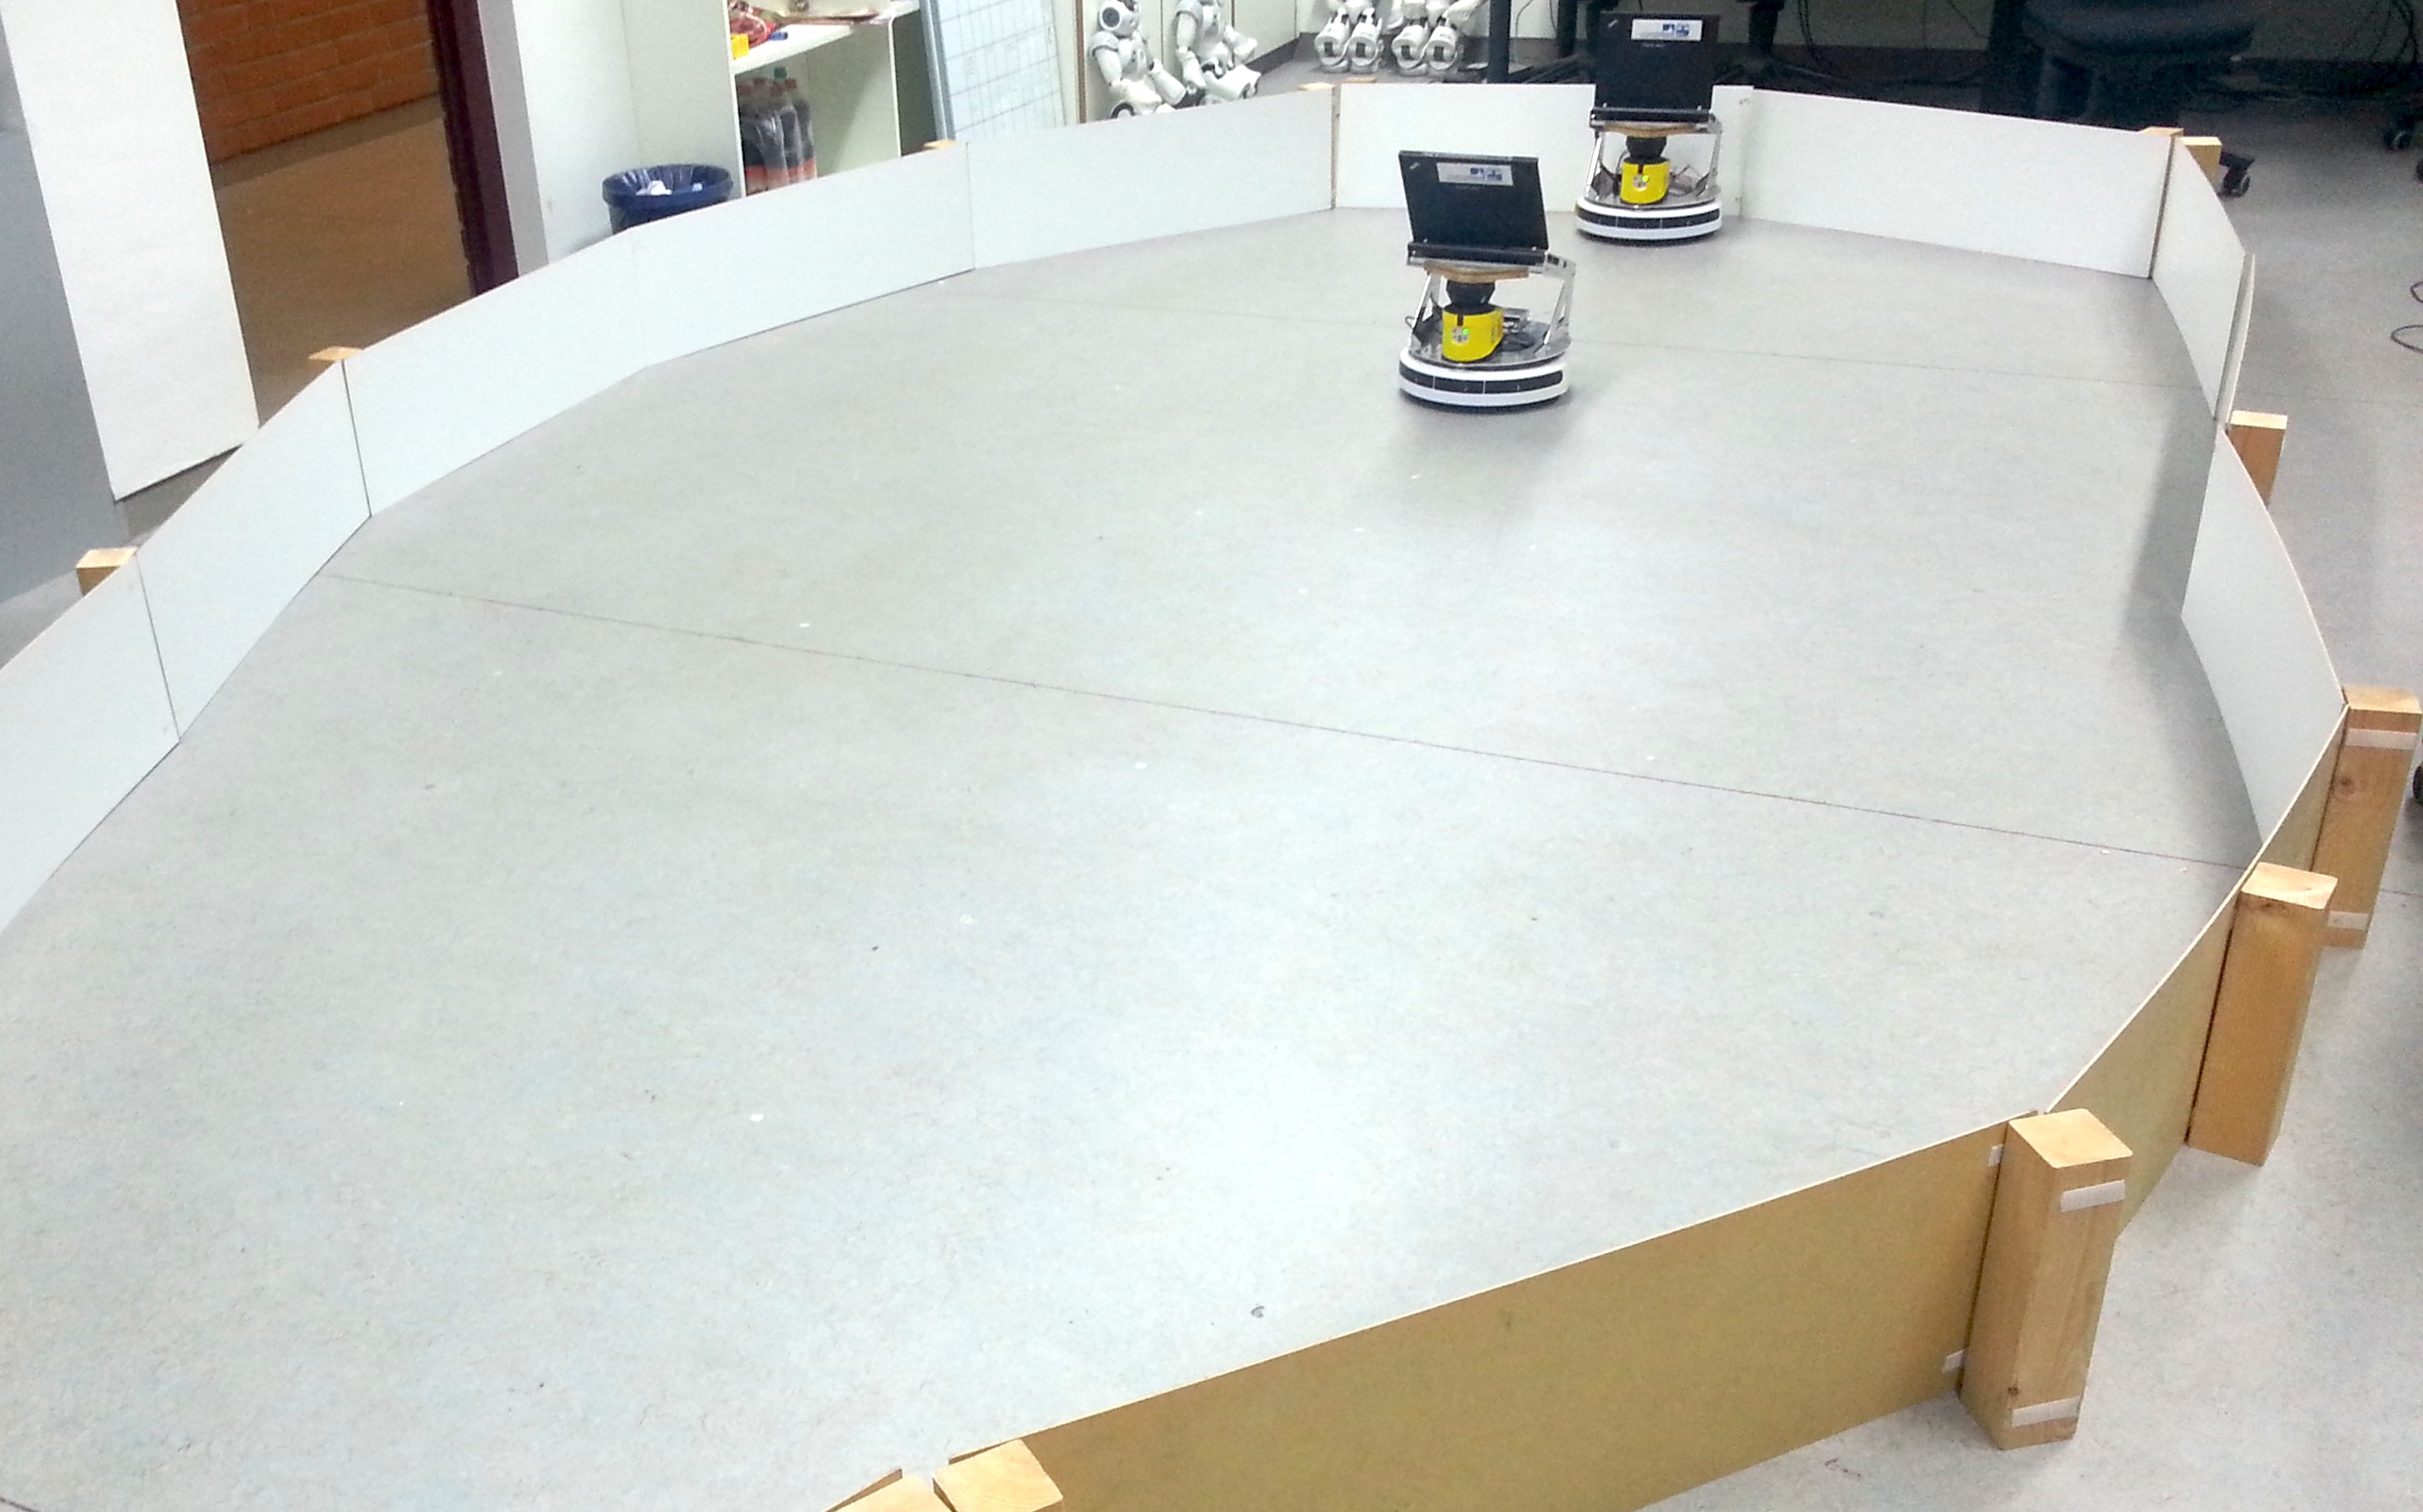
\includegraphics[width=0.95\textwidth]{img/test_setup.jpg}
		\caption{Test Setup Environment}
			\label{fig:test_setup}
	\end{figure}

	For these four tests, the robot with the \intrudy system was always in the same starting position, but the robot with the target system had its position changed in each test. The ``target'' robot had the same behaviour in all enviroments: move forward at the speed of 0.25 m/s until an obstacle is detected, then halt. The four initial positions of the ``target'' were:

	\begin{enumerate}
		\item The ``target'' was 1 meter away from the \intrudy robot and both robots had the same orientation.
		\item The ``target'' was 4 meters away from the other robot and the robots were facing each other.
		\item The ``target'' was 1 meter to the left and 2 meter to the front of the \intrudy robot. With respect to \intrudy's coordinate system, the target robot was looking at 0\degrees while \intrudy was looking
		at 90\degrees.
		\item Similar to the third test but the target robot was at the right side this time looking with an angle of 180\degrees with respect to \intrudy's coordinate system.
	\end{enumerate}
	
	The last five tests had the same robot initial position as the first test, but they were done in the following enviroments:
	
	\begin{enumerate}[start=5]
		\item The mobile robotics lab without any plywood simulating the walls, with many obstacles present, such as chairs and table legs.
		\item The hallway in front the mobile robotics lab without any obstacles, but with doorways present. 
		\item The hallway T-shaped intersection near the previously mentioned lab.
		\item The octagonal room near the lab, which had chairs, metal objects and glass doors as challenges.
		\item The octagonal room, but with plywood covering the chairs and the glass doors.
	\end{enumerate}

	% subsection tests_setup_and_description (end)

	\subsection{Qualitative Results} % (fold)
	\label{sub:qualitative_results}
	
		In all the tests the \intrudy robot managed to follow the ``target'', but in most of the cases it has stopped several times during the following process. 

		Four aspects of the test results were taken in account during the
		qualitative evaluation of the robot: 
		\begin{enumerate}
			\item Did \intrudy follow the target, i.e., did it constantly move towards the target?
			\item Did \intrudy find the target frequently, i.e., was \intrudy able to reacquire the target while moving
			and stopped less times.
			\item Did \intrudy stop after the target stopped?
			\item Did \intrudy stop close to the final target's position?
		\end{enumerate}
		This aspects were evaluated during the tests with four possible values:
		\begin{itemize}
			\item it does sometimes (\cmark),
			\item it does constantly (\cmark\cmark),
			\item it does it one or two times (\xmark),
			\item it does not do it at all (\xmark\xmark).
		\end{itemize}
		
		The obtained qualitative results are shown in Table~\ref{tab:qualitative_results}.


		\begin{table}
			\center
			\begin{tabular}{|c|c|c|c|c|}
				\hline 
				Test & Aspect 1 & Aspect 2 & Aspect 3 & Aspect 4\tabularnewline
				\hline 
				\hline 
				1 & \cmark\cmark & \xmark & \cmark & \cmark\cmark\tabularnewline
				\hline 
				2 & \cmark\cmark & \cmark & \cmark & \cmark\cmark\tabularnewline
				\hline 
				3 & \cmark\cmark & \cmark\cmark & \xmark & \xmark\tabularnewline
				\hline 
				4 & \cmark & \xmark & \xmark\xmark & \xmark\xmark\tabularnewline
				\hline 
				5 & \cmark\cmark & \cmark & \xmark & \xmark\xmark\tabularnewline
				\hline 
				6 & \cmark\cmark & \cmark & \cmark\cmark & \cmark\tabularnewline
				\hline 
				7 & \cmark\cmark & \cmark & \cmark\cmark & \cmark\tabularnewline
				\hline 
				8 & \cmark\cmark & \cmark\cmark & \cmark\cmark & \cmark\cmark\tabularnewline
				\hline 
				9 & \cmark\cmark & \cmark & \xmark & \cmark\tabularnewline
				\hline 
			\end{tabular}
			\caption{Qualitative results of the nine tests}
			\label{tab:qualitative_results}
		\end{table}

		The test number 8, in the octagonal room, prooved to be the best one qualitative speaking even though this enviroment contained more obstacles and objects that creates more noise in the sensors.

		% subsection qualitative_results (end)

		\subsection{Quantitative Results} % (fold)
		\label{sub:quantitative_results}

		Since the quantitive results are not enough to determine how good the system is, the scans and changes in the the system states were logged . This logs were parsed afterwards to obtain some measurements to compare each test and to see if the system actually is doing what it is suppose to do. The measurements done are the following: 
		\begin{itemize}
			\item Time needed for initial detection.
			\item Difference between last time it was found and last time the target moved.
			\item Number of times the target was found in each of the states.
			\item Number of times the target was not found in each of the states.
		\end{itemize}

		Also, the accuracy should be one of the measurements done to this result, but due to time limitations it was not done. The results can be observed in Table~\ref{tab:intrudy_quantitive_tests} and in Figure~\ref{fig:intrudy_success_and_fail}.

		\begin{table}
			\center
			\begin{tabular}{|c|c|c|}
				\hline 
				Test & Initial Detection & Diff. of last movement and last time found\tabularnewline
				\hline 
				\hline 
				1 & 0.94 secs & 5.26 secs\tabularnewline
				\hline 
				2 & 7.13 secs & 4.5 secs\tabularnewline
				\hline 
				3 & 0.76 secs & 6.59 secs\tabularnewline
				\hline 
				4 & 0.96 secs & 4.30 secs\tabularnewline
				\hline 
				5 & 0.90 secs & -5.80 secs\tabularnewline
				\hline 
				6 & 1.05 secs & -0.97 secs\tabularnewline
				\hline 
				7 & 1.0 secs & -3.76 secs\tabularnewline
				\hline 
				8 & 1.07 secs & 0.27 secs\tabularnewline
				\hline 
				9 & 0.98 secs & 2.93 secs\tabularnewline
				\hline 
			\end{tabular}
			\label{tab:intrudy_quantitive_tests}
		\caption{Quantitive results of the nine tests}
		\end{table}
		

		\begin{figure}
			\center
			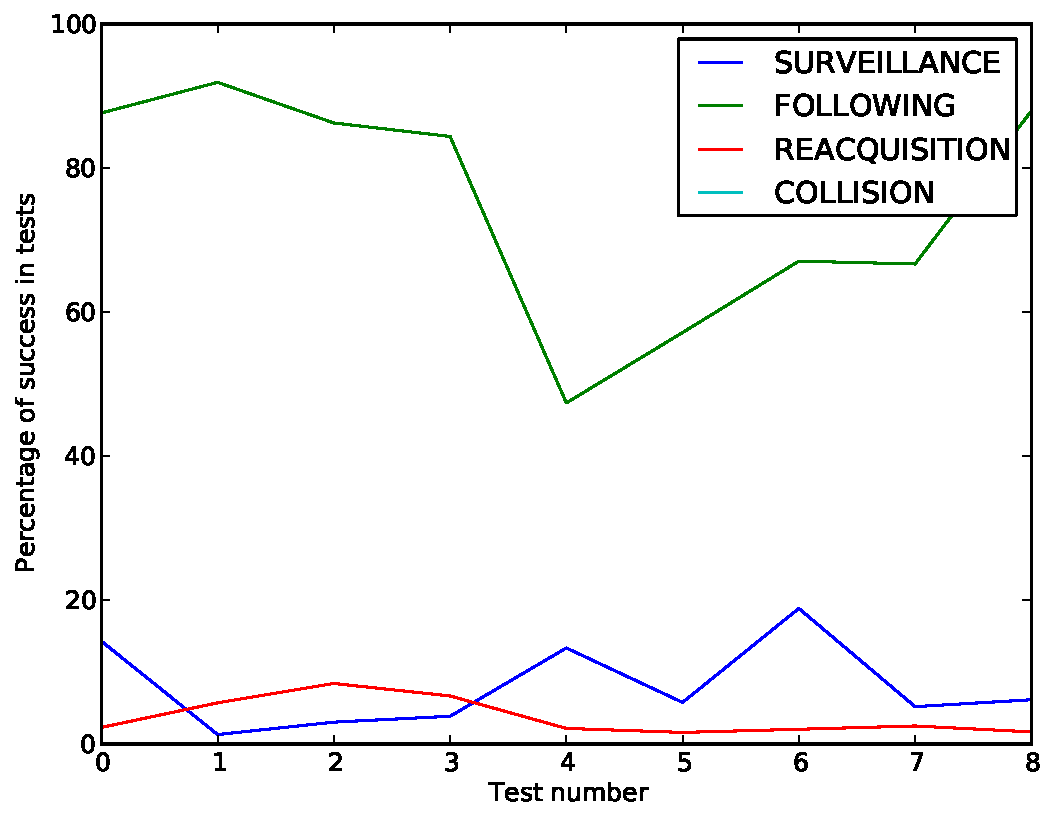
\includegraphics[width=0.49\textwidth]{img/plot1}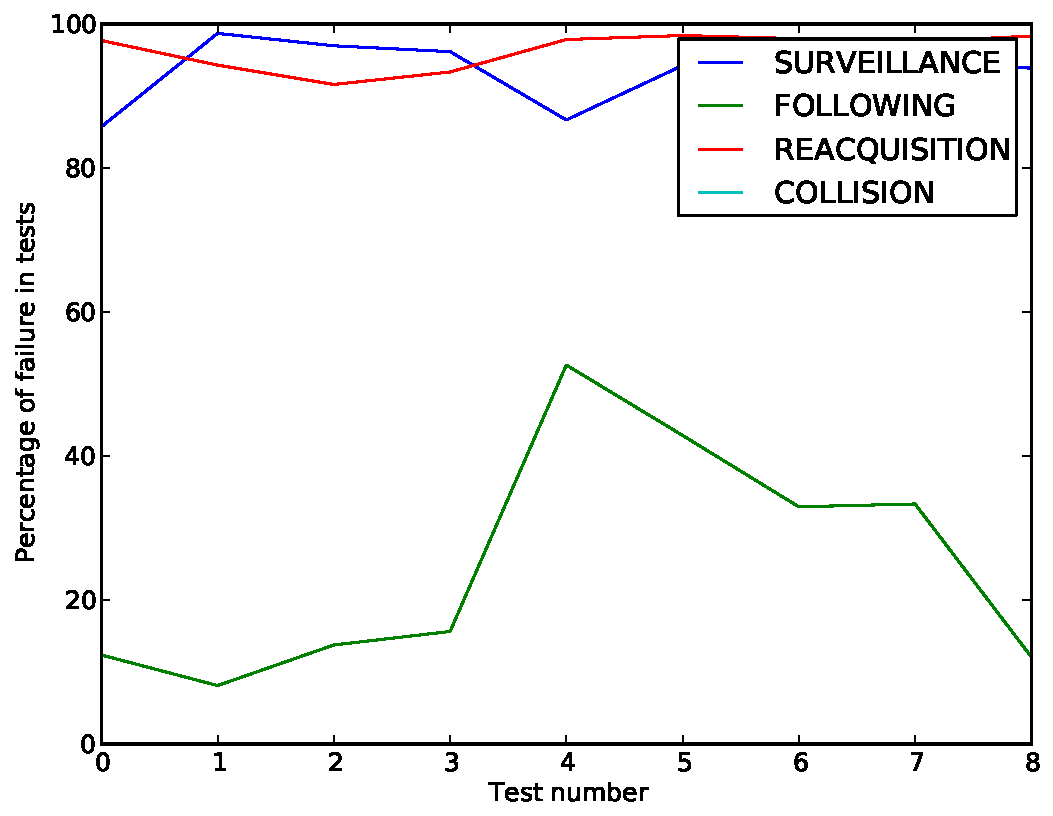
\includegraphics[width=0.49\textwidth]{img/plot2}
			\caption{Percentage of the times \intrudy found the target successfully	(left) and unsuccessfully (right) for each state}
			\label{fig:intrudy_success_and_fail}
		\end{figure}


		% subsection quantitative_results (end)
	
% section evaluation_of_results (end)

\newpage

\section{Future development} % (fold)
\label{sec:future_development}
Even though the current implementation of \intrudy achieves the goals set for it, it is not completely an error-prone implementation. In this section we will propose a set of steps to be taken in future to improve the performance of \intrudy with respect to the evaluation described in section~\ref{sec:evaluation_of_results}.

At the current implementation status, the system has difficulties following the target continuously. Several parts of the algorithm could be changed in order to achieve a better performance. This report will mention three of these possible changes.
\begin{enumerate}
	\item Better ICP implementation: One of the several variations of the ICP algorithm can be used to obtain better results when aligning the two scans. This will yield a more accurate target and will permit the user to increase the sensibility of the system.

	\item Reduce the effect of the noise in the target detection: During the analysis of the results it was observed that several of the scans contained faulty measurements: the maximum range value.

	\item Increase the search window in the re-acquisition mode for each time step: Increasing this window size will enable \intrudy to find the target that moves faster than we expected, or that was not found in several time steps and that still continued moving during the re-acquisition phase.
\end{enumerate}
Also, a better obstacle avoidance algorithm can be implemented to aid better overall performace of \intrudy.
% section future_development (end)


% BIBLIOGRAPHY
\newpage
\bibliographystyle{plain}
\bibliography{bibliography}

\end{document}

